\documentclass{article}

\usepackage{amsfonts} 
\usepackage{amsmath} 
\usepackage{graphicx} 
\usepackage{float} 
\usepackage{natbib} 
\usepackage{slashbox} 
\usepackage{graphicx} 
\usepackage{flushend} 
\usepackage{amsmath} 
\usepackage{amssymb} 
\usepackage{amsxtra} 
\usepackage{amstext} 
\usepackage{amsthm} 
\usepackage{amsbsy} 
\usepackage{latexsym} 
\usepackage{mathrsfs} 
\usepackage{eucal} 
\usepackage{synttree} 


\usepackage[spanish]{babel}
\usepackage[utf8x]{inputenc}
\author{Flores González Luis Brandon - 312218342 \\ García Argueta Jaime Daniel - 312104739 \\ Tarea 2. Modelo Entidad – Relación}
\title{}
\date{01 de marzo de 2017}


\begin{document}

	\maketitle	
	
	\begin{enumerate}
		\item \textbf{Repaso de conceptos generales}
			\begin{enumerate}
				\item Un conjunto de \textbf{entidades débiles} siempre se puede convertir en un conjunto de \textbf{entidades fuertes}
				añadiéndole a sus atributos la \textbf{llave primaria} del conjunto de entidades fuertes a las que está
				asociado. Describe qué tipo de redundancia resultaría si se realizara dicha conversión.
				\\\\Por redundancia entendemos al almacenamiento de los mismos datos varias veces en diferentes lugares. En este caso tendríamos el mismo valor(llave primaria) tanto en la entidad fuerte como en la débil(fuerte cuando se agregue) esto produciría los siguientes inconvenientes:
					\begin{itemize}
						\item Incremento de trabajo: como un mismo dato está almacenado en dos o más lugares, esto hace que cuando se graben o actualicen datos, deban hacerse en todos los lugares a la vez.
						\item Desperdicio de espacio de almacenamiento, ya que los mismos datos están almacenados en varios lugares distintos.
						\item Inconsistencia de datos: esto sucede cuando los datos redundantes no son iguales entre sí. Esto puede suceder, por ejemplo, cuando se actualiza el dato en un lugar, pero el dato duplicado en otro lugar no es actualizado.\\
					\end{itemize}
				\item Responde a las siguientes cuestiones, deberás indicar \textbf{si son posibles o no}, justificando tu
				respuesta. Cuando no sea posible deberás indicar alguna recomendación al respecto:
				\begin{itemize}
					\item ¿Un \textbf{atributo compuesto} puede ser \textbf{llave}?
					\\Si, este se designa como llave además todos los atributos componentes de la llave compuesta deben estar incluidos para tener la propiedad de unicidad. 
					\item ¿Un \textbf{atributo multivaluado} puede ser \textbf{llave}? 
					\\No, ya que debe ser único.
					\item ¿Un \textbf{atributo derivado} puede ser \textbf{llave}? 
					\\No, ya que el valor no es estático. Un ejemplo puede ser que se calcule una edad a partir de una fecha, este cambiara. 
					\item ¿Un \textbf{atributo multivaluado} puede ser \textbf{compuesto}? 
					\\Si, ya que cada valor puede estar compuesto. Por ejemplo un nombre que esta en un atributo multivaluado.
					\item ¿Un \textbf{atributo multivaluado} puede ser \textbf{derivado}? 
					\\Si, por ejemplo una fecha de nacimiento.
					\item ¿Qué implicaría la existencia de una \textbf{entidad} cuyos atributos sean \textbf{todos derivados}?				
					\\En caso de que no haya otra entidad, no sería posible ya que no habría un atributo del cual derivar. Pero si existiera tal entidad los costos serían muy superiores.\\
				\end{itemize}
				\item Explica el concepto de \textbf{agregación} en el \textbf{modelo E/R} y proporciona un par de ejemplos.
				\\\\Es una abstracción a través de la cual las relaciones se tratan como entidades de un nivel más alto. Se utiliza para expresar relaciones entre relaciones o entre entidades y relaciones. Se representa englobando la relación abstraída y las entidades que participan en ella en un rectángulo.\\
					\begin{figure}[H]
					\centering
					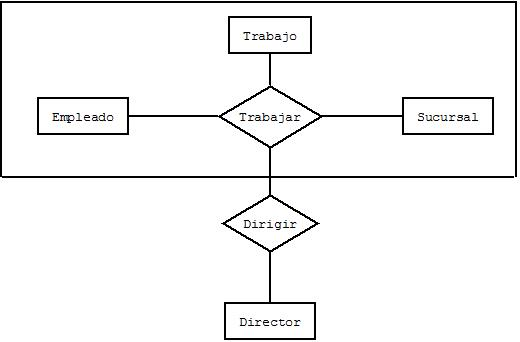
\includegraphics[width=1\textwidth]{imagenes/Agregacion1}
					\caption{Ejemplo 1}
					\end{figure}
					\begin{figure}[H]
						\centering
						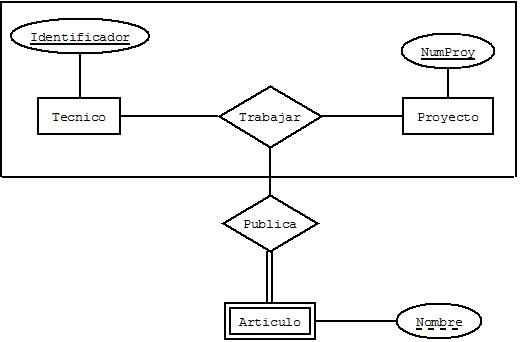
\includegraphics[width=1\textwidth]{imagenes/Agregacion2}
						\caption{Ejemplo 2}						
					\end{figure}
				\item Diseña un \textbf{modelo E/R} en donde reflejes los conceptos vistos para el tema de \textbf{Modelo E/R} (no
				tienes que considerar el modelo E/R extendido).
				\\\\Se necesita administrar la información de los grupos de una escuela, estos necesitan conocer la información de sus profesores tal como nombre, edad, etc. Además se necesita conocer las materias que imparten, queda claro que todo profesor imparte al menos una materia. Además se necesita conocer tanto los alumnos que pertenecen a un grupo como los profesores que le dan clase a esos alumnos.
				\begin{figure}[H]
					\centering
					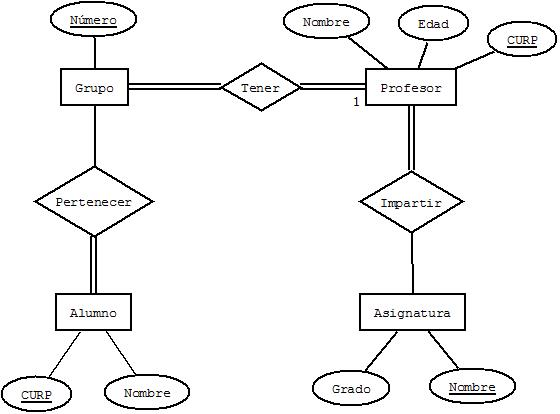
\includegraphics[width=1\textwidth]{imagenes/EjemploDiagrama}										
				\end{figure}				
			\end{enumerate}
		\item \textbf{Modelo Entidad/Relación}
			\begin{enumerate}
				\item \textbf{Venta de automóviles}
				\\Se desea construir una base de datos para una agencia de venta de autos, la cual requiere tener control de las ventas que realiza, así como los trabajadores que laboran en ella.
				Para los trabajadores requiere almacenar: \textbf{nombre, CURP, fecha de nacimiento, sueldo, fecha de ingreso a la agencia} y su \textbf{dirección}. Necesita además almacenar información específica para los distintos trabajadores:		
				\begin{itemize}
					\item Vendedores $\rightarrow$ comisión.
					\item Asesor de ventas $\rightarrow$ los accesorios que vende.
					\item Guardias de seguridad $\rightarrow$ su turno y área.
					\item Limpieza $\rightarrow$ el turno que labora así como el área.
				\end{itemize}		
			Es importante paras la agencia tener información de sus clientes para próximas ofertas. En este
			caso se necesita conocer: \textbf{nombre, CURP, fecha de nacimiento, dirección} y la \textbf{forma de pago}; si el
			cliente pide un \textbf{crédito} a la agencia, se necesita tener un \textbf{control de los pagos} (el total de monto
			a financiar, la fecha de las parcialidades y el monto) para que en todo momento se pueda
			conocer la deuda actual. En cuanto a las agencia solo se necesita almacenar: \textbf{el nombre, RFC y
			la dirección donde se ubica}. Se pide considerar que se trata de una empresa en expansión y que,
			en algún momento, puede haber más de una sucursal operando a lo largo de la república.
			\\\\\\ \textbf{El diagrama se encuentra al final en orden respectivo.}\\\\		
			\item \textbf{Juego de computadora}
			\\Se desea construir una base de datos para modelar \textbf{un juego de
			computadora}. En el juego se utilizan conceptos como: \textbf{personajes,
			objetos} y \textbf{escenarios}. Las especificaciones del diseño son:
				\begin{itemize}
					\item Cada \textbf{personaje} tiene un nombre único y lleva asociados \textbf{5 valores}
					que indican: \textbf{vida, nivel de fuerza, inteligencia, habilidad y rapidez}.
					Interesa saber cada momento en qué escenario se encuentra. Cada
					personaje tiene un rol en el juego (p.e. enemigos, aliados, etc.) y cada
					personaje puede dominar a otros personajes (a cero o más), pero sólo
					puede ser dominado por otro, o por ninguno.
					\item Los personajes tienen en cada momento algunos \textbf{objetos} en su poder. Los objetos pueden
					incrementar alguna de sus características (p.e. pócimas para aumentar la fuerza) o bien puede
					ser armas. Cada objeto tiene un \textbf{nombre} y un \textbf{tipo}, además de un valor numérico que indica el
					porcentaje en que puede incrementar una característica o bien el daño en el nivel de vida que
					puede reducir.
					\item Además de saber qué objetos tiene cada personaje hay que guardar información acerca de
					en qué momento (\textbf{hora, minuto y segundo}) tomó el personaje el objeto. Puede haber objetos
					que no estén en posesión de ningún personaje (no los ha encontrado nadie aún), pero ninguno
					puede pertenecer a dos personajes al mismo tiempo.
					\item Los objetos se deben poder distinguir entre sí y están determinados por el escenario en que se
					encuentran situados al comienzo del juego. Cada escenario puede contener 0 o más objetos.
					\item Cada escenario es único y tiene 2 factores: \textbf{riesgo y tiempo}, mismos que indican características
					particulares del escenario en que el jugador se ubique.
					\item Se deben almacenar todas las estadísticas del juego para cada jugador, como, por ejemplo,
					\textbf{nombre del jugador, puntos alcanzados, nivel de avance, tiempo de juego}, y algún aspecto
					adicional que se considere pertinente.\\\\
					
				\end{itemize}
			\textbf{El diagrama se encuentra al final en orden respectivo.}\\\\
			
			
			\item \textbf{Sitio social de fotografías}
			\\Hoy en día, son muy populares los sitios web sociales que almacenan
			fotografías (p. e. \textbf{Instagram}) y eres contratado para realizar un sitio similar
			considerando las siguientes características:
				\begin{itemize}
					\item Los \textbf{usuarios} que se registran en el sitio tienen \textbf{nombre de usuario,
					contraseña, correo electrónico, un nombre real, un alias y una fecha de
					nacimiento}. Todos los usuarios deben tener una \textbf{foto de perfil} e interesa
					mantener un histórico de todas las fotos que han sido elegidas para este fin.
					\item Los usuarios pueden subir cualquier \textbf{número de fotografías} y es importante
					para los usuarios saber el número de fotografías que se han publicado en el sitio.
					\item Una fotografía tiene un \textbf{nombre, un identificador, una fecha y hora} en que se subió al sitio, \textbf{título
					y descripción}. Los usuarios pueden crear \textbf{álbumes} con las fotografías que ha subido, los álbumes tienen un \textbf{nombre y una fecha de creación}; un usuario no puede tener álbumes con nombres
					repetidos, pero dos distintos usuarios podrían tener un álbum con el mismo nombre.
					\item Los usuarios pueden \textbf{calificar las fotos} de cualquier otro usuario. Los usuarios pueden marcar
					fotos como favoritas.
					\item Los usuarios pueden ser \textbf{amigos de otros usuarios}, los cuales pueden ser \textbf{familiares, compañeros
					de trabajo o amigos} (reales y/o virtuales). Los usuarios pueden dejar \textbf{comentarios} en las
					fotografías y un mismo usuario puede realizar varios comentarios.\\\\
				\end{itemize}
			\textbf{El diagrama se encuentra al final en orden respectivo.}\\\\
			\end{enumerate}
		\item \textbf{Ingeniería inversa.}
			\begin{figure}[H]
				\centering
				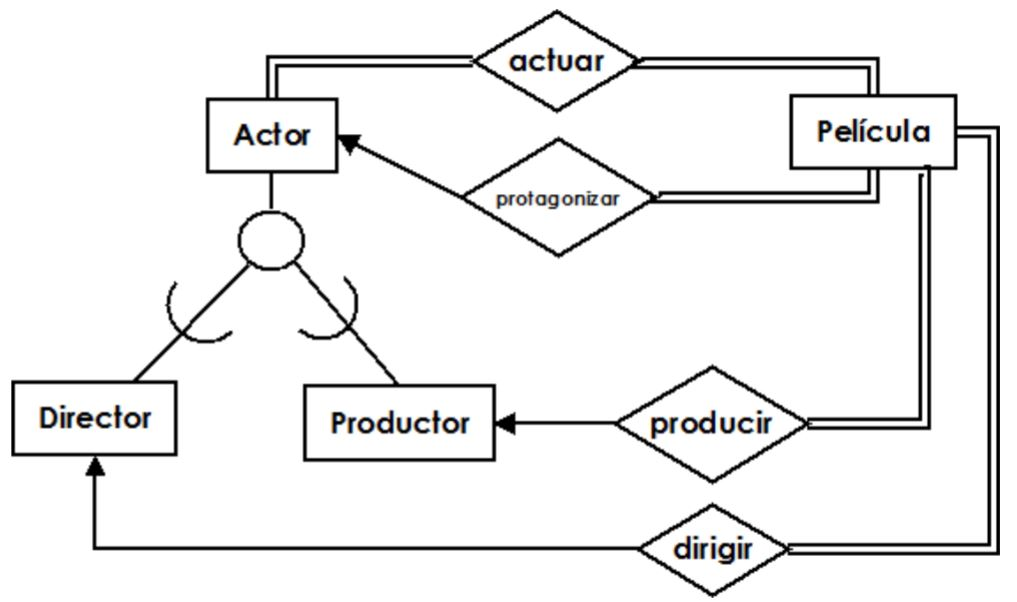
\includegraphics[width=1\textwidth]{imagenes/IngenieraInversa}
				\caption{Base de datos Películas.}
			\end{figure}
			\begin{itemize}
				\item En esta base de datos no hay ningún actor que no haya actuado en ninguna película.
				\\\\Verdadero, ya que hay al menos un actor que haya actuado en al menos una película.\\
				\item Hay algunos actores que han actuado en más de diez películas.
				\\\\Quizá, ya que debe haber al menos uno que haya actuado pero no podemos saber la cantidad de cuantas peliculas a actuado.\\
				\item Algunos actores han sido protagonistas en varias películas.
				\\\\Quiza, ya que algunos pudieran haber no protagonizado varias peliculas o algunos pudierón protagonizar varias peliculas.\\				
				\item Una película sólo puede tener un máximo de dos protagonistas.
				\\\\Falso ya que un actor puede protagonizar varias peliculas, y puede haber mas de dos actores.\\
				\item Cada director ha sido actor en alguna película.
				\\\\Falso, ya que puede haber aunque sea uno que no haya actuado.\\
				\item Ningún productor ha sido actor alguna vez.
				\\\\Quiza, ya que la participación es parcial.\\
				\item Un productor no puede ser actor en alguna otra película.
				\\\\Falso, ya que la cardinalidad es de muchos a muchos.\\
				\item Hay películas con más de una docena de actores.
				\\\\Quiza, ya que la cardinalidad es de muchos a muchos.\\
				\item Algunos productores también han sido directores.
				\\\\Quiza, ya que esta expresado con traslape. Es decir, puede ser director y productor\\
				\item La mayoría de las películas tienen un director y un productor.
				\\\\Verdadero, ya que de la de entidad película a la relación producir y dirigir la participación es total.\\ 
				\item Algunas películas tienen un director, pero varios productores.
				\\\\Falso, ya que la cardinalidad de directo y productor es 1 a muchos.\\
				\item Hay algunos actores que han interpretado el papel de protagonista, dirigido una película y
				producido alguna película.
				\\\\Quiza, ya que las sub-entidades no son disjuntas y hay un relación hacía todas estas.\\
				\item Ninguna película tiene un director que también haya actuado en ella.
				\\\\Quiza, ya que la especialización es paracial y puede que se cumpla esta condición o no.\\
			\end{itemize}
	\end{enumerate}
\end{document}